\chapter{Types de données Abstraits (TAD)}
\minitoc
C'est une méthode de spécification de structures de données(SD).

C'est utile pour la programmation << En large >>, c'est-à-dire à plusieurs, pour cela nous sommes obligés de travailler sur la communication et
l'échange sur le code produit, on utilise pour cela les \textbf{spécifications} : 
\begin{itemize}
	\item Les Entrées Sorties du programme \footnote{Vu au S3}
	\item Les données\footnote{Nous nous occuperons de cette partie}
\end{itemize}
\begin{figure}[H]
	\centering
	\includegraphics[width=8cm]{content/schemas/schemaTAD.eps}
	\caption{Principe de base d'un TAD}
\end{figure}
\exemple{\textbf{Les entiers}

\begin{description}
	\item[Utilisateur: Représentation Interne] 1, 2, 3, + ,-, /, +, \%
	\item[Programmeur: Représentation Externe] Entiers << machine >> 0000 0011 pour le 3
\end{description}
}

\section{Syntaxe des TAD}
La syntaxe d'un TAD est répartis en deux étapes : 
\begin{description}
	\item[La signature du TAD\footnote{signature de base}] Donner les interfaces de la données
	\item[La sématique abstraite du TAD\footnote{signature étandue}] Décrire logiquement le fonctionnement de la données.\\
		Une donnée c'est une ou un ensemble de valeurs mais aussi les opérations qui permettent de la manipuler. Cette étape étape nous donne : 
		\begin{itemize}
			\item Les limitations de la donnée (préconditions)
			\item Les descriptions longueur du fonctionnement de chaque opération
		\end{itemize}
\end{description}
\subsection{Signature du TAD \texttt{Pile}}\label{pileStatique}
Une pile est unee structure de données qui permetn de rassembler des éléments de telle sorte que le dernier élément entré dans la pile soit le premier à
en sortir.\footnote{Last In First Out}.
\paragraph{Signature de base}
\begin{description}
	\item[Sorte] Pile
	\item[Utilise] Élément, Booleen 
	\item[Opérations]~ 
		\begin{description}
			\item[\texttt{creer}] $\rightarrow$Pile % CONSTRUCTEURS
			\item[\texttt{empiler}] Pile $\times$ Element $\rightarrow$ Pile
			\item[\texttt{estVide}] Pile $\rightarrow$ Booleen  %% OPERATEURS
			\item[\texttt{sommet}] Pile $\rightarrow$ Pile
			\item[\texttt{appartient}] Pile $\times$ Element $\rightarrow$ Booleen 
		\end{description}
\end{description}

\paragraph{Signature étandue}
\begin{description}
	\item[Préconditions]~
		\begin{itemize}
			\item \texttt{sommet(p)}$\Leftrightarrow$ $\neg$ \texttt{estVide(p)}
		\end{itemize}
	\item[Axiones]~
\end{description}
~\newline
Avant toute chose, on partitionne l'ensemble des opérations en deux sous ensembles: 
\begin{itemize}
	\item Les constructeurs
	\item Les opérateurs
\end{itemize}
L'ensemble des constructeurs est nécessaire et suffisant pour pouvoir gagner n'importe quelle valeur de la donnée
\begin{lstlisting}[language=C, numbers=none,caption=Opérations du TAD Pile]
// On applique chaque constructeur à chaque opérateur et on decrit logiquement 
// ce qu'il se passe
estVide(creer()) = true;
estVide(empiler(p, x)) = false;
depiler(creer()) = creer();
depiler(empiler(p, x)) = p;
sommet(empiler(p, x)) = x;
appartient(creer(), x) = false;
appartient(empiler(p, x), y) = (x = y) $\vee$ appartient(p, y)
 \end{lstlisting}

\section{Implémentation d'un TAD}
\begin{enumerate}
	\item Implémenter la structure de données
	\item Implémenter les opérateurs
	\item Séparer l'interface du corps des opérations
		\begin{description}
			\item[But 1] Permet de modifier les opérations sans remettre en cause la manière d'utiliser le TAD
			\item[But 2] Protéger les données
		\end{description}
\end{enumerate}

\subsection{Implémentation de la structure de données et des opérateurs}
Trouver une représentation interne de la structure de données, celle-ci est contrainte par le langage choisi.

Celle-ci peut être statique ou dynamique.
\begin{description}
	\item[Statique] La donnée ne peut plus changer de place ni de taille mémoire ou dynmaique.
		\begin{itemize}
			\item Problème de gaspillage de place
			\item Avantage de l'efficacité
		\end{itemize}
	\item[Dynamique] La donnée peut changer de taille ou de place pendant l'execution du programme.
		\begin{itemize}
			\item Pas de gaspillage de place
			\item Inconvénient de l'efficacité
		\end{itemize}
\end{description}

\section{Protection du TAD}
La protection d'un TAD se fait en deux phases : 
\begin{description}
	\item[séparer corps - interface] Bibliothèque 
	\item Protéger le type
\end{description}
\subsection{Séparation du corps et de l'interface}
	Cela correspond à une biblitohèque, ainsi nous allons séparer le fichier source en trois fichiers : 
	\subsubsection{Fichiers}
	\begin{description}
		\item[\texttt{fichier.h}] Contient les prototypes de fonctions et les \texttt{typedef}.
		\item[\texttt{fichier.c}] Contient \texttt{\#include ''fichier.h''} et les implémentations de fonctions sauf le main.
		\item[\texttt{testFichier.c}] Contient \texttt{\#include ''fichier.h''} et le \texttt{main}.
	\end{description}
	\subsubsection{Compilation}	
	\begin{itemize}
		\item \texttt{gcc -c fichier.c}
		\item \texttt{gcc -c testFichier.c}
		\item \texttt{gcc fichier.o testfichier.o -o nomExe}
	\end{itemize}
	\subsection{Protection du type}
	Nous allons étudier le cas de la pile statique.

\begin{lstlisting}[language=C, numbers=none,caption=Type de la pile statique originel -- Présent dans le .h]
#define N 1000
typedef struct etPile {
	element tab[N];
	int nb;
} Pile;
\end{lstlisting}

Nous allons devoir cacher ce type afin que l'utilisateur ne le modifie pour cela, il sera caché dans le .c et un pointeur présent dans le .h.
\begin{lstlisting}[language=C, numbers=none,frame=none, caption=Type de la pile statique -- Présent dans le .h]
typedef struct etPile* pile;
\end{lstlisting}
\begin{lstlisting}[language=C, numbers=none,caption=Type de la pile statique -- Présent dans le .c]
#define N 1000
typedef struct etPile {
	element tab[N];
	int nb;
}Pile;
\end{lstlisting}

Nous devons ainsi modifier le fichier source afin d'utiliser le pointeur sur pile.
\begin{lstlisting}[language=C, numbers=none,caption=Modification de la fonction \texttt{creer} s'adaptant à la protection de données]
	Pile p;
	p = (Pile)malloc(sizeof(PileInterne));
	p->nb = 0

	return p;
\end{lstlisting}

\remarque{Désormais nous ferons systématiquement la séparation corps - interface et la protection du type.}
